\documentclass[12pt]{article}
 
\usepackage[margin=1in]{geometry} 
\usepackage{amsmath,amsthm,amssymb}
\usepackage{hyperref}
\usepackage{graphicx}
\usepackage{xcolor}
\usepackage[many]{tcolorbox}
\tcbuselibrary{listings}
\usepackage{listings}
\usepackage{float}

\definecolor{lg}{HTML}{f0f0f0}

\newtcblisting{pycode}{
    colback=lg,
    boxrule=0pt,
    arc=0pt,
    outer arc=0pt,
    top=0pt,
    bottom=0pt,
    colframe=white,
    listing only,
    left=15.5pt,
    enhanced,
    listing options={
        basicstyle=\small\ttfamily,
        keywordstyle=\color{blue},
        language=Python,
        showstringspaces=false,
        tabsize=2,
        numbers=left,
        breaklines=true
    },
    overlay={
        \fill[gray!30]
        ([xshift=-3pt]frame.south west)
        rectangle
        ([xshift=11.5pt]frame.north west);
    }
}

\lstset{
    language=Python,
    basicstyle=\small\ttfamily,
}

 
\begin{document}
 
\title{Exercise 4}
\author{Cristian Manuel Abrante Dorta - 888248\\
ELEC-E8125 - Reinforcement Learning}

\maketitle
\section{Approximation with non-linear features}

\subsection{Task 1}
\textbf{Implement Q-learning using function approximation, at every timestep using the latest state transition to perform a TD(0) update. Test the implementation on the
Cartpole environment. Test two different features for state representations}\\

For the implementation of function approximation using TD(0) update, the following formula was used for updating the target ($\delta$) values of the stochastic gradient regressor:

\begin{equation}
    \delta = r + \gamma \cdot max_a {Q(\phi(s'), a)}
\end{equation}

Where:

\begin{itemize}
    \item $r$: is the reward obtained in the current state.
    \item $\gamma$: is the discount factor for future actions.
    \item $\phi(s)$: is the featurizer function, in this task two different functions were used.
    \item $max_aQ(\phi(s'), a)$: is the maximum value function of the next state, following the optimal policy.
\end{itemize}

Using this formula, and for the two featurizer functions, the following plots were obtained:

\begin{figure}[H]
    \centering
   \begin{minipage}{0.48\textwidth}
     \centering
     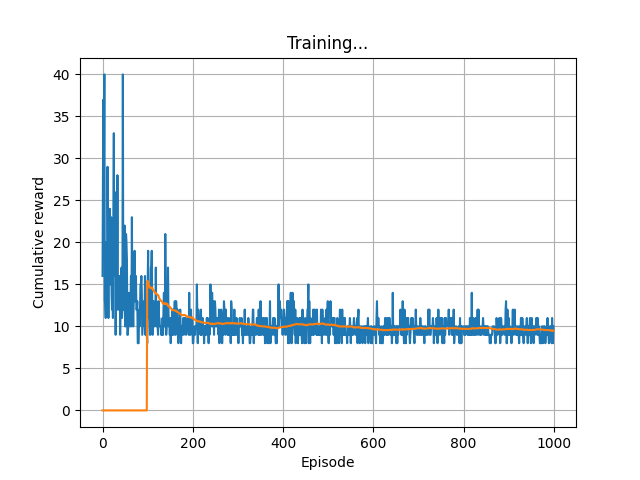
\includegraphics[width=0.9\linewidth]{exercise-4/plots/task-1a.png}
     \caption{Plot for handcrafted feature vector}
     \label{fig:task-2-1}
   \end{minipage}\hfill
   \begin{minipage}{0.48\textwidth}
     \centering
     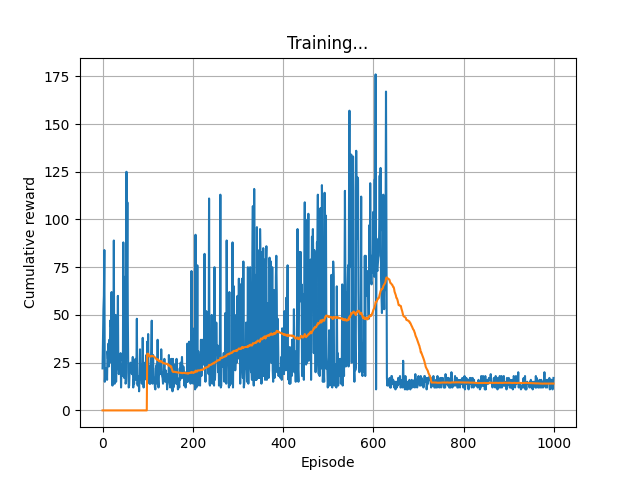
\includegraphics[width=0.9\linewidth]{exercise-4/plots/task-1b.png}
     \caption{Plot for radial basis function representation}
     \label{fig:task-2-2}
   \end{minipage}
\end{figure}

As we can see in this plots, the second function allows the agent to actually learn the underlying pattern, on the contrary, using the first feature vector, the model is not able to learn. 

\subsection{Question 1}
\textbf{
Would it be possible to learn accurately Q-values for the Cartpole problem using linear features (by passing the state directly to a linear regressor)? Why/why not?
}\\

There are some reasons that would make difficult to learn accurately the Q-values for the Cartpole environment if we pass directly the state to the linear regressor. \\

The main drawback of doing this, is that the state is not scaled by default, and that would make more difficult for the regressor to learn the weights. For overcoming this first difficulty, the value of the states has been scaled using an standard scaler, fitted with an arbitrary dataset created with a range of possible values. \\

The second drawback of passing the state directly is that it only contains 4 values, so the regressor would only have four weights for features. This could be not enough information for the generalization of the Q values.

\subsection{Task 2}
\textbf{Modify your Task 1 implementation to perform minibatch updates and use experience replay (while keeping the original code for Task 1 submission). Run the experiments with Cartpole with both feature representations.}\\

Using minibatch updates and experience replay, Task 1 was executed, obtaining the following plots as a result:

\begin{figure}[H]
    \centering
   \begin{minipage}{0.48\textwidth}
     \centering
     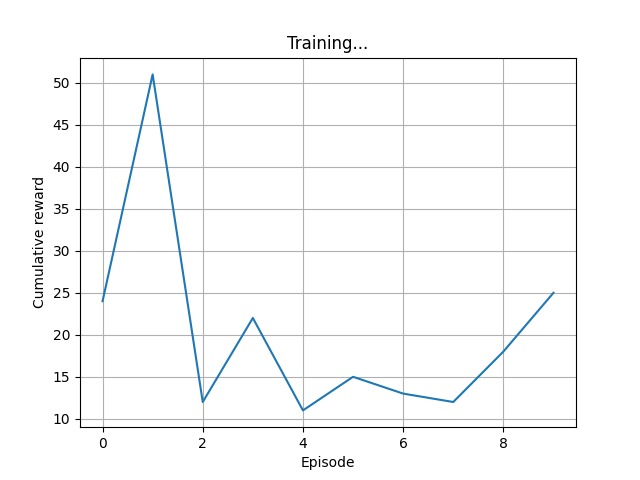
\includegraphics[width=0.9\linewidth]{exercise-4/plots/task-2a.png}
     \caption{Minibatch and experience replay with handcrafted vector}
     \label{fig:task-2-1}
   \end{minipage}\hfill
   \begin{minipage}{0.48\textwidth}
     \centering
     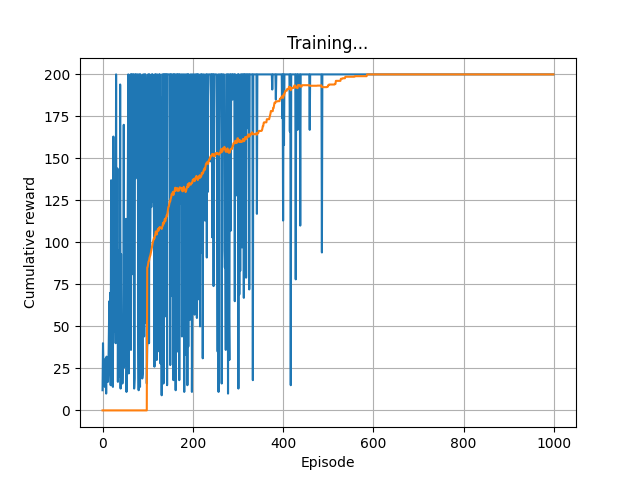
\includegraphics[width=0.9\linewidth]{exercise-4/plots/task-2b.png}
     \caption{Minibatch and experience replay with radial basis function representation}
     \label{fig:task-2-2}
   \end{minipage}
\end{figure}

As we can see, experience replay and minibatch perform extremely well, achieving almost the higher possible reward from episode 500. On the other hand, even though we apply minibatch and experience replay, the handcrafted feature vector have not performed really well.

\subsection{Question 2}
\textbf{
Figure 2 shows the training performance of all four methods from Task 1, together with grid-based learning from Exercise 3 evaluated using GLIE with $\alpha = 50$.
}

\subsubsection{Question 2.1}
\textbf{How does the experience replay affect the learning performance?}\\

Experience replay when applied to the handcrafted feture vector and the RBF featurer really makes a difference. We can see that the agent is able to reach higher rewards in early episodes. This is significant with handcrafted vector, because with experience replay we can see that the agent is able to reach the 50 timesteps of reward in almost the begining on the training, while it takes almost 500 episodes to be reached without it. Something similar happens with RBF, where the curve of the rewards is always better until almost 600 episodes. \\

On the other hand, we can see that in the last episodes the experience replay curves overperform compared to the algorithm withouth experience replay. This could be due to the overfitting of the regressor, which alllows it to perform well in the early stages but decrease its performance in the final epochs.

\subsubsection{Question 2.2}
\textbf{Discuss the benefits and cons of using hand-crafted features.}

The main advantage of using handcrafted vectors is the simplicity of understanding and implementation. One example of that, is the easy implementation of the transformation $|s|$. Other advantage of them is that usually they are computationally efficient to compute, because they are composed of basic operations.\\

On the other hand, the main drawback of them is that they could sometimes not contain as much information of the state as the agent needs to generalize the desired value or behaviour, this is why sometimes, other methods such as radial basis functions are used.

\subsubsection{Question 2.3}
\textbf{
Do grid based methods look sample-efficient compared to any of the function approximation methods? Why/why not?
}\\

Grid based methods look sample-efficient according to the plot, mainly because they reach the stability in earlier stages compared to the other algorithms. But apart from being sample-efficient, they seem not improve to better rewards when this stability is reached.

\subsection{Task 3}
\textbf{Create a 2D plot of policy (best action in terms of state) learned with RBF
with experience replay in terms of x and $\theta$.} \\

The heatmap created for the representation, shows the two possible actions (0 and 1, correspondent to move left and right), for a discretized version of 16 steps, both for $x$ and $\theta$:

\begin{figure}[h]
    \centering
    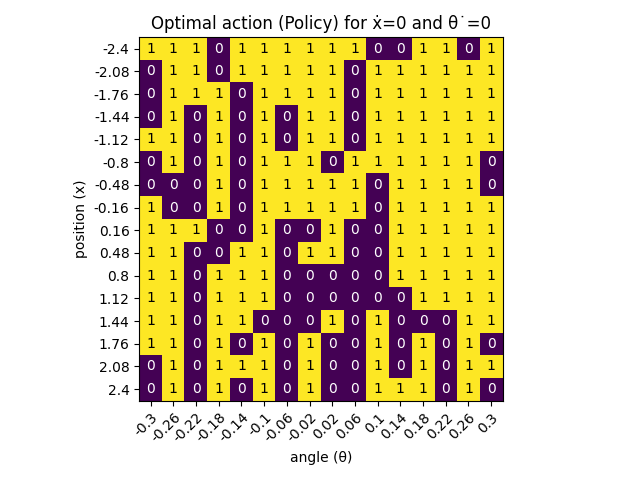
\includegraphics[scale=0.75]{exercise-4/plots/task-3.png}
    \label{fig:my_label}
\end{figure}


\bibliographystyle{ieeetr}
\bibliography{template}  % Modify template with your bibliography name
\end{document}
